% Should be <2 pages


\section{Data Reading Rate}
\subsection{Behaviors}

\begin{figure}[H]
\centering
	\begin{subfigure}[b]{0.3\textwidth}
    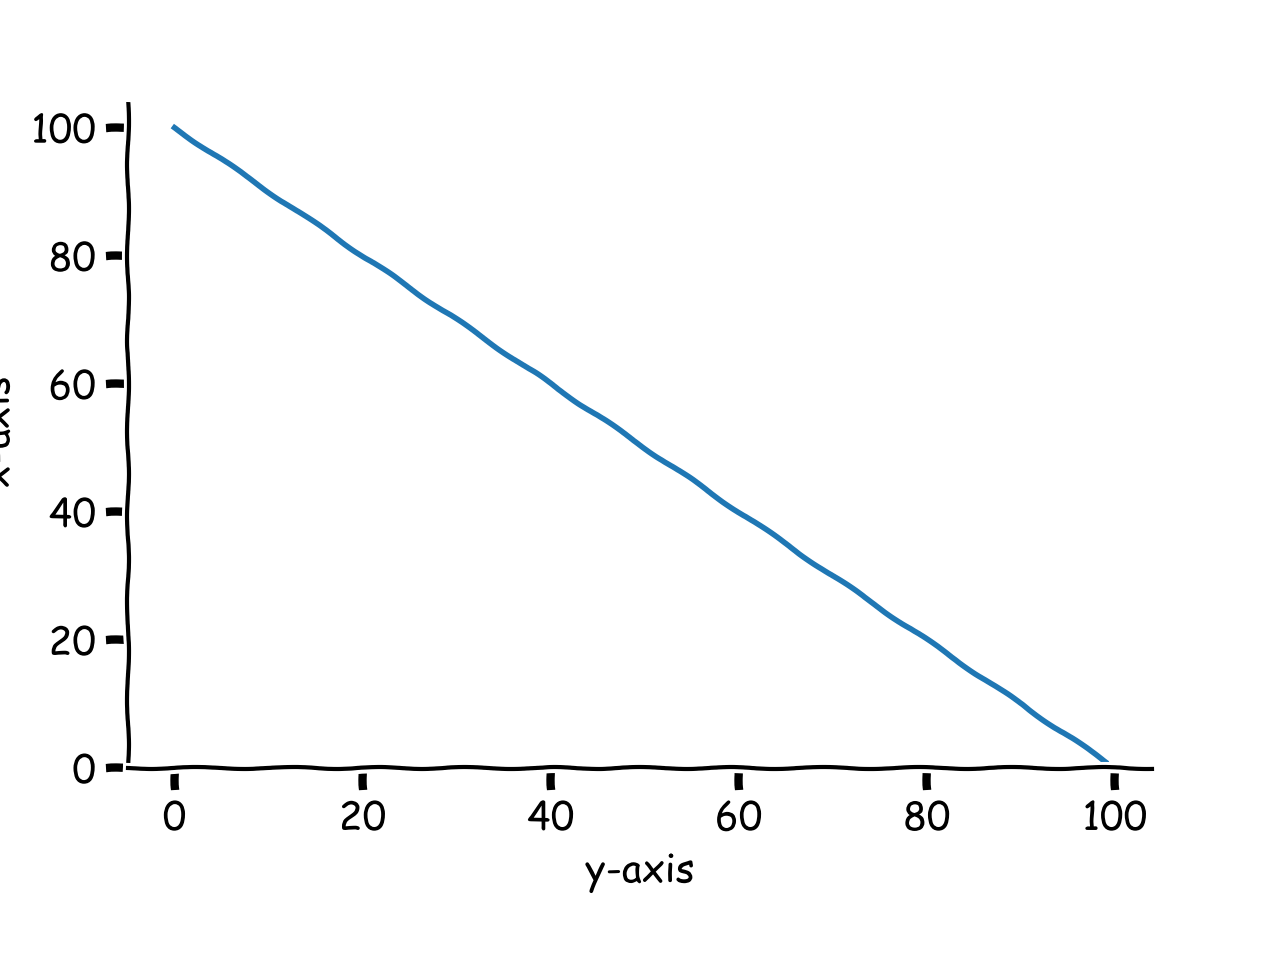
\includegraphics[width=\textwidth]{linear.png}
    \caption{Graph with linear decrease}
    \label{fig:linear}
	\end{subfigure}
	%
	\begin{subfigure}[b]{0.3\textwidth}
    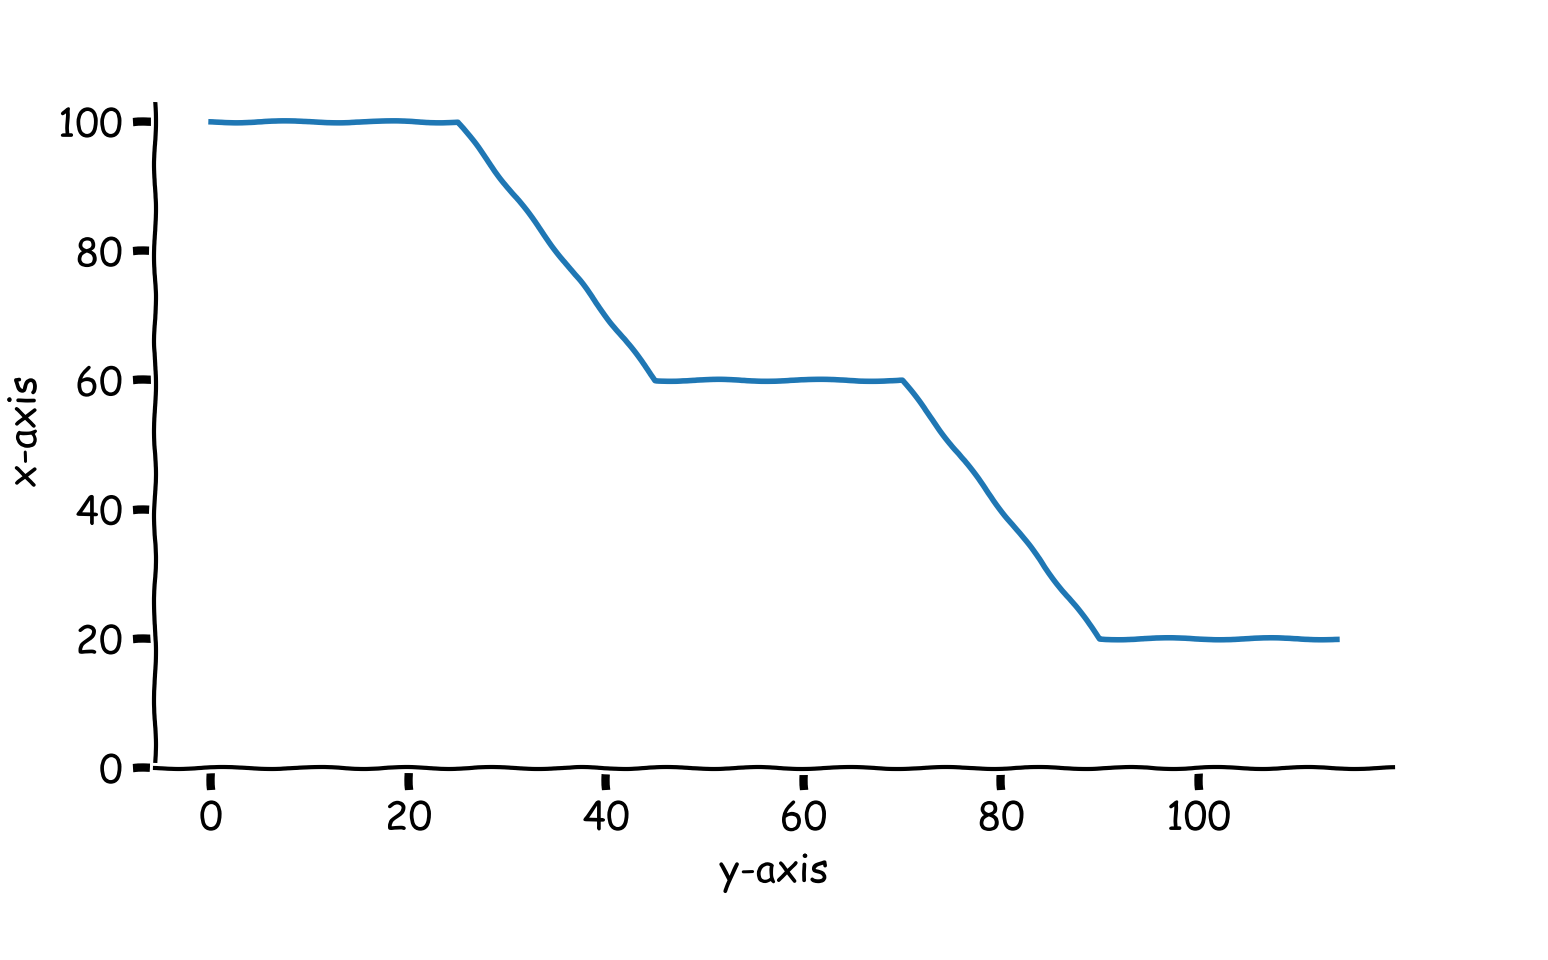
\includegraphics[width=\textwidth]{plateu.png}
    \caption{Graph with plateaus}
    \label{fig:plat}
	\end{subfigure}
	%
	\begin{subfigure}[b]{0.3\textwidth}
    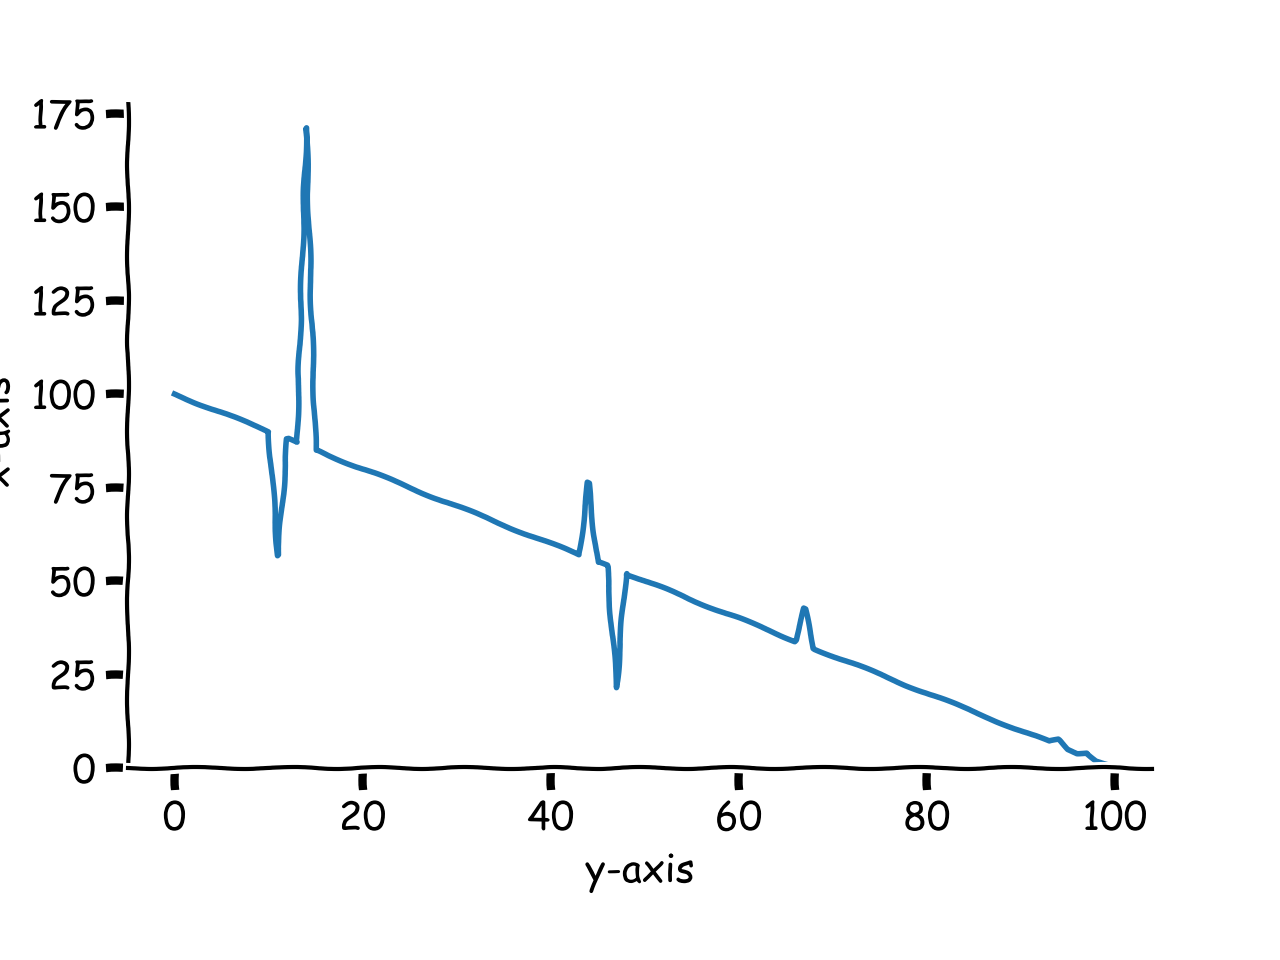
\includegraphics[width=\textwidth]{spikes.png}
    \caption{Graph with spikes}
    \label{fig:spikes}
	\end{subfigure}
\end{figure}

To determine what we want to achieve in this aspect, it's useful to first define some behaviors from which we will base our assumptions on. In figure \ref{fig:linear} we see our base case, with a simple linear decline in data values. In figure \ref{fig:plat} we see data the goes through some changes periodically, but stabilizes itself between the changes. In figure \ref{fig:spikes} we see a clear linear decrease with some spikes in data values here and there, which we can assume to be faulty measurements.

\subsection{Implementation}
We're interested in modifying the data reading rate depending on the changes in data values. This can be done in a number of ways, but a simple start might be to measure the delta in the last \textit{x} amount of values and increase/decrease the rate depending on it's relation to delta. 

To do this we need a \textit{short term buffer} of a fixed size that contains \textit{x} amount of recently read values in chronological order. This buffer should act as a FIFO-queue, so that the first element added to the buffer is the first one removed during an overflow. Measuring the delta of all the values in the buffer, we compare it to a threshold value that will either decrease, increase or maintain the current interval of reading data. When we say the delta of \textit{all} values in the buffer, we mean the delta between each data point summed up. Assuming a buffer of 10 values, we would calculate the sum as follows:

$$\sum_{n=0}^{8} x_n - x_{n+1}$$

Starting with figure \ref{fig:linear}, the values go from (100-0) in 100 data points on the x-axis. Calculating the delta for the first 10 values would be simple. The short term buffer would be: [100, 99, ..., 91]. The total delta would be (100-99) + (99 - 98) + ... + (92 - 91) = 10. For this example we can say that our determined threshold for decreasing our reading interval is $\geq 15$, and an increase at $\leq 5$. In our current example the reading rate is maintained. 

In figure \ref{fig:plat} the slopes are steeper, and would thus generate a larger total delta. Assuming a buffer length of 10, the first 5 values would be 100, and the other 5 would be 75. Our delta calculation would give us a value of 25, which would warrant a increase in our reading rate. In figure \ref{fig:spikes} the calculation would work the same as as in \ref{fig:linear}, with the exception of some outlying data points. In regards to data reading rate, we can handle these values in two ways. Either we filter them in some way, or include them. Depending on the application, filtering can be easy. For example, perhaps we know that values $\geq$ 150 are impossible for our sensor, and thus we can manually check each values to see if they adhere to our specific bounds. Perhaps we know that such rapid changes in said values aren't possible, and we can filter them based on that. One way of doing this might be to calculate the average value of the short term buffer, and only allow new data within a range of  \textit{x} amount of units. Given the short term buffer [100, 99, ... 91], the average value would be 95.5. In our application we know that data points can only reasonably change with about ~20 units, assuming a minimum reading rate. We set the limit to 30 units to give the program some leeway. In either way, extreme data points can be filtered. 

A valid question at this point is \textit{how often} we should perform this delta measurement, and of course the answer depends on the needs and workings of the application. Some applications might benefit from adjusting their reading rate very tightly, while others might only want to do this periodically. 

To sum up the important design choices when considering how often the sensor should be polled, we considered:
\begin{itemize}
	\item What values we \textbf{compare} our short-term delta to. When should we decrease, increase or maintain our current data reading rate.
	\item What values are \textbf{valid} in the context of our application.
	\item How \textbf{often} we should adjust our reading rate interval.
\end{itemize}

\section{Sensor Failure}

\subsection{Behaviors}
In this paper we define

\section{Sensor Disconnect}